\section{\textit{Encoders} Incrementais}
\label{sec:encoders}
% Referencias:
% https://www.roboticsbusinessreview.com/news/differences-between-encoder-resolution-accuracy-and-precision/
% https://www.newtoncbraga.com.br/index.php/como-funciona/5454-mec128
% [Speed Measumment Using Rotary encoders for High Performance ac Drives]
% [Speed Measurement Algorithms for Low-Resolution Incremental encoder Equipped Drives: a Comparative Analysis]
% [A Simple Speed Feedback System for Low Speed DC Motor Control in Robotic Applications]
% [An Embedded System for Position and Speed Measurement Adopting Incremental encoders]

% FALAR SOBRE O FUNCIONAMENTO BASICO
% CITAR OS DIFERENTES TIPOS
% FALAR DO GRAY CODE
% FALAR DO ERRO DE QUANTIZAÇÃO

As saídas de um \emph{encoder} incremental são, normalmente, duas ondas quadradas defasadas em $90^\circ$ uma da outra (em quadratura). Essa diferença de fase nos permite medir o sentido de rotação. Abordagens mais eficientes de leitura desses sensores são por meio da detecção das bordas dessas ondas, pois isso permite quadruplicar o número de pulsos por revolução (NPR) \cite{quantization_error01}. Existem dois métodos básicos para se realizar a medição da velocidade por meio desses sensores, são eles: \textbf{frequencímetro} e \textbf{periodímetro}. 

Na medição por frequência (\textbf{frequencímetro}), conta-se o número de pulsos que ocorreram em um determinado período de tempo fixo. Com isso a velocidade pode ser obtida pela seguinte aproximação:

\begin{equation}
    \omega = \frac{d\theta}{dt} \cong \frac{\Delta{\theta}}{T} \cong \frac{2 \pi \Delta{N}}{N_{PR}T}[rad.s^{-1}] \xrightarrow{} \frac{60 \Delta{N}}{N_{PR} T} [RPM]
\end{equation}

Sendo $N_{PR}$ o número de pulsos por revolução e $\Delta{N}$ é o número de pulsos que aconteceram dentro da janela de tempo $T$. Existe um erro de quantização nesse método de leitura devido à variação de ângulo medida ser sempre um múltiplo inteiro de $ 2\pi/N_{PR}$. O erro de quantização $\Delta{\omega}$ pode ser modelado pela seguinte equação:

\begin{equation}
    \Delta{\omega} = \frac{2\pi}{N_{PR}T}[rad.s^{-1}] \xrightarrow{} \frac{60}{N_{PR}T}[RPM]
    \label{eq:erro_de_quantizacao_frequencimetro}
\end{equation}

\begin{figure}[H]
    \centering
    
\includegraphics[width=0.5\textwidth]{figuras/ilustracoes/ilustracao_erro_de_quantizacao.eps}
    \caption{Ilustração do erro de quantização na medição de velocidade de rotação.}
    \label{fig:ilustracao_erro_quantizacao}
    \fonte{Própria.}
\end{figure}

A Figura \ref{fig:ilustracao_erro_quantizacao} ilustra um exemplo de medição de velocidade com erro de quantização.\\

Nota-se pela Equação \ref{eq:erro_de_quantizacao_frequencimetro} que o erro de quantização para a medição por frequência decresce com o aumento do número de pulsos por revolução e/ou com o aumento da janela de tempo ($T$), porém o aumento do período de observação acrescenta um atraso na medição da velocidade. O erro relativo à velocidade pode ser descrito como a seguir:

\begin{equation}
    e_{\omega} = \frac{2\pi}{\omega N_{PR} T}
    \label{eq:erro_relativo_quantizacao_frequencimetro}
\end{equation}

Pela Equação \ref{eq:erro_relativo_quantizacao_frequencimetro} observa-se que o erro relativo decresce conforme a velocidade $\omega$ aumenta, ou seja, o erro de quantização será mais significante para baixas velocidades.\\

\begin{figure}[H]
    \centering
    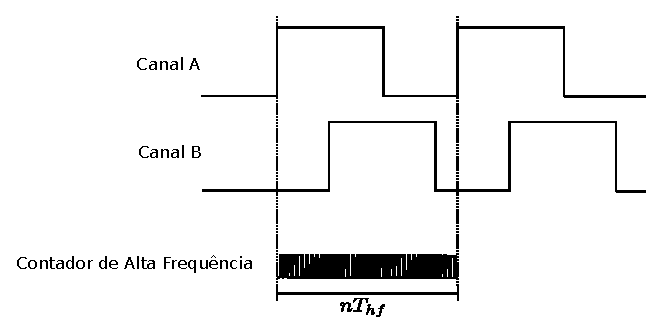
\includegraphics[width=0.5\textwidth]{figuras/ilustracoes/ilustracao_medicao_encoder_por_periodo.eps}
    \caption{Ilustração de leitura de \emph{encoder} periódica.}
    \label{fig:ilustracao_periodimetro}
    \fonte{Própria.}
\end{figure}

O outro método de leitura dos \emph{encoders} incrementais é por medição de intervalos de tempo de um mesmo pulso (\textbf{periodímetro}) (ver Figura \ref{fig:ilustracao_periodimetro}). A seguinte formulação pode ser obtida considerando a velocidade do motor constante e sem levar em conta o sentido de giro:

\begin{equation}
    \omega = \frac{d\theta}{dt} \cong \frac{\Delta{\theta}}{nT_{hf}} \cong \frac{2\pi}{N_{PR} n T_{hf}} [rad.s^{-1}] \xrightarrow{} \frac{60}{N_{PR} n T_{hf}} [RPM]
    \label{eq:omega_periodimetro}
\end{equation}
onde $T_{hf}$ é o período do sinal do contador de alta frequência do microcontrolador e $n$ é a quantidade de pulsos, desse contador, que ocorreram entre os pulsos dos \emph{encoder}.

O período entre pulsos será:

\begin{equation}
    T_{\omega}(\omega) = \frac{2\pi}{N_{p}\omega} [s]
\end{equation}

Uma aproximação para o pior caso do erro de quantização relativo a velocidade é apresentado a seguir \cite{analise_incr_enc}:

\begin{equation}
    e_{\omega} = \frac{T_{hf}}{ \frac{2\pi}{N_{PR} \omega} - T_{hf} } \cong \frac{\omega N_{PR} T_{hf}}{2\pi}
    \label{eq:erro_quantizacao_periodimetro}
\end{equation}

A Equação \ref{eq:erro_quantizacao_periodimetro} mostra que o erro é diretamente proporcional à velocidade e a quantidade de pulsos por revolução ($N_{PR}$) e decresce com o aumento da frequência do contador de alta frequência (diminuição de $T_{hf}$).\\

Nesta versão do trabalho, foi adotada a medição da velocidade pelo método do periodímetro, devido ao fato do método do frequencímetro apresentar erros maiores em baixas velocidades, que normalmente são as situações onde se precisa de um controle mais preciso, e consequentemente de uma medição mais confiável. O método do periodímetro pode apresentar erro maior em altas velocidades, mas em compensação disponibiliza muitas medidas dentro de um mesmo ciclo de controle, que podem ser fundidas pelo filtro de Kalman e gerar um resultado estimado com baixo erro.\\

Já para se obter o \textbf{sentido da velocidade $\omega$} é necessário fazer uso do padrão binário gerado pelas bordas dos sinais em quadratura. A Figura \ref{fig:cw_signal} ilustrado os sinais em quadratura para uma rotação no sentido horário e destaca o padrão binário gerado nas bordas. A Figura \ref{fig:ccw_signal} ilustra os sinais no sentido anti-horário. O padrão de dois bits é apresentado na Tabela \ref{tab:tabela_simple_code}. \\

\begin{figure}[H]
    \centering
    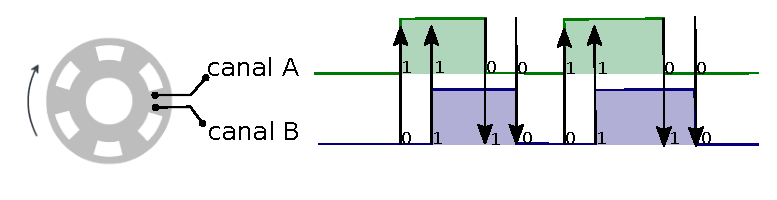
\includegraphics[width=0.7\textwidth]{figuras/ilustracoes/sinal_enquadratura_sentido_CW.eps}
    \caption{Sinal em quadratura para rotação no sentido horário.}
    \label{fig:cw_signal}
    \fonte{Própria.}
\end{figure}

\begin{figure}[H]
    \centering
    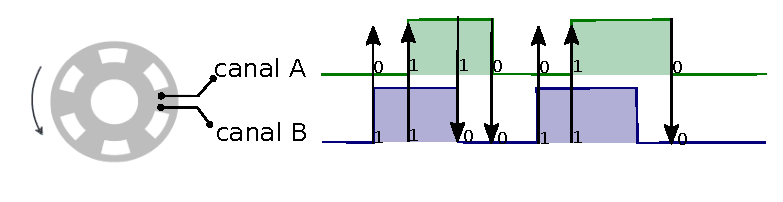
\includegraphics[width=0.7\textwidth]{figuras/ilustracoes/sinal_enquadratura_sentido_CCW.eps}
    \caption{Sinal em quadratura para rotação no sentido anti-horário.}
    \label{fig:ccw_signal}
    \fonte{Própria.}
\end{figure}

% Please add the following required packages to your document preamble:
% \usepackage{graphicx}
\begin{table}[H]
\centering
\resizebox{0.5\textwidth}{!}{%
\begin{tabular}{cc|cc}
\multicolumn{2}{c|}{\textbf{\begin{tabular}[c]{@{}c@{}}Sentido\\     Horário\end{tabular}}} &
  \multicolumn{2}{c}{\textbf{\begin{tabular}[c]{@{}c@{}}Sentido\\ Anti-Horário\end{tabular}}} \\ \hline
\textbf{A} & \textbf{B} & \textbf{A} & \textbf{B} \\
1          & 0          & 0          & 1          \\
1          & 1          & 1          & 1          \\
0          & 1          & 1          & 0          \\
0          & 0          & 0          & 0         
\end{tabular}%
}
\caption{Código de 2 bits para identificar o sentido de rotação.}
\label{tab:tabela_simple_code}
\end{table}


\begin{comment}
% Speed Measumment Using Rotary encoders
% for High Performance ac Drives

SPEED MEASUREMENT USING A PERIODIMETER

If we use a periodimeter, we will get the speed not by counting pulses from the encoder, but by counting a high frequency (HF) clock

Let $\alpha_p$ be the corresponding angle to the higher part of an encoder pulse (half of its period), t the period of the HF clock, and n the number of HF pulses arrived at the HF counter. Then, the time spent on an encoder pulse, $T_e$ is:

\begin{equation}
    T_e = n t
\end{equation}

Rotor speed can be obtained as:

\begin{equation}
    \omega_{rotor} = \frac{\alpha_p}{T_e}
\end{equation}

As with the frequencimeter, here also there is a quantization error because of the time T,, which will be always an integer multiple of t With a fixed HFclock frequency, this error will increase as n decreases, that is, as the encoder rotates faster, but it provides accurate measurements at lower speeds. Because the variable with quantization noise is now in the denominator, its effects are much more important than in the frequencimeter.

An additional advantage at low speed is that, as it only needs one pulse to get the speed, the delay is minimal, which is very important at lower speeds.

It also possible to use quadruple frequency. Of course, this reduces the precision, and therefore the maximum velocity where this method is suitable, but also, and this is much more important, it reduces the delay obtaining the velocity when the motor works at low speed. Nevertheless, this method produces stability problems in the zero speed cross. Figure 8 shows an inversion with two possible situations in the encoder output signals. Supposing that there is no quadruple frecuency, and PHASE A controls the HF counter, we see that at the encoder pulse end, the counter has a wrong value, because about half of the HF pulses arrived on each direction of rotation.

The accuracy of the periodimeter is, more than the frequencimeter, related to the accuracy of the encoder, which in general depends on the errors in the radial grating, and the eccentricity of the graduated disk to the bearing.

% Speed Measurement Algorithms for
% Low-Resolution Incremental encoder Equipped
% Drives: a Comparative Analysis


At very low speed the number of high frequency pulses can be extremely high and saturation of the digital timer employed for measurement can occur. Also a speed sample is not available each speed control period, needing an adaptation of the control parameters. In that situation, the quadrature decoding of the encoder pulses can be exploited in order to reduce the width of the measuring window by a factor of four or a reduction of the frequency of the timer can be considered.

The former solution allows to reduce the speed sampling period and improve the control performance of the drive, but makes the measuring system more sensitive to sensor nonidealities, including variations in the transition locations from their nominal values and phasing errors between encoder channels. When low-cost and low-resolution sensors are employed, nonidealities play the major role in the determination of period measuring errors and has to be carefully analysed in drive design phase. The latter solution needs to switch on-line the frequency of the timer and adapt the coeffients of the equations above.

The implementation of the period measuring method is also straightforward as it requires a simple timer capture unit, commonly found inside recent microcontrollers.

% A Simple Speed Feedback System for Low Speed
% DC Motor Control in Robotic Applications

The relationship between the measured frequency using PIC microcontroller and the percentage error is shown in Fig. 2. The percentage error is given as:

\begin{equation}
    e\% = \frac{F_m - F_a}{F_a}.100
\end{equation}

where F m and F a denote the measured and actual frequencies. It is observed that as the frequency increases, the error in the frequency measured from PIC increases linearly, that is, there is a linear relationship between error and frequency.

\end{comment}